\documentclass{beamer}
\mode<presentation> 
{
	\usetheme[alternativetitlepage]{Torino}
	\usecolortheme{chameleon}
	\setbeamercovered{transparent}	
}
\definecolor{olive}{RGB}{51, 149, 48}
\definecolor{red}{RGB}{195, 2, 36}

\usepackage{ucs}
\usepackage[utf8x]{inputenc}
\usepackage[czech]{babel}
\usepackage{palatino}
\usepackage{graphicx}
\usepackage{epstopdf}
\usepackage{color}
\usepackage[export]{adjustbox}
\usepackage{multicol}
\usepackage{hyperref}
\usepackage[labelfont={color=olive,scriptsize}]{caption}
\usepackage{subcaption}
\usepackage{amsmath}



\title{\large{\textbf{Postprocessing OpenGL scény}}}

\author{Pavel Macenauer \\ \tiny{xmacen02@stud.fit.vutbr.cz} \\ \normalsize{Jan Bureš} \\ \tiny{xbures19@stud.fit.vutbr.cz}}
\date{\tiny{\today}}
\institute[FIT VUTBR]
{
	\inst{}
	Fakulta Informačních Technologií \\
	Vysoké Učení Technické v Brně
}

\begin{document}

	\begin{frame}[t,plain]
	\titlepage

	\vspace{-7mm}
	\center{ 
\includegraphics[height=7mm]{logo.eps} }
	\end{frame}

	%% ------------- Obsah projektu -------------

	\begin{frame}[t,fragile]
		\frametitle{\textbf{Obsah projektu}}	
		\Large
		\begin{itemize}
			\item vyrenderování OpenGL scény do textury
			\item vyrenderování této textury na obrazovku
			\item postprocessing
		\end{itemize}
	\end{frame}
	
	%% ------------- Framebuffer Object -------------

	\begin{frame}[t,fragile]
		\frametitle{\textbf{Framebuffer Object}}
	
		\begin{itemize}
			\item kombinace color, depth, stencil bufferů
			\item základní OpenGL kontext má výchozí framebuffer, lze vytvořit i vlastní
			\item \verb|glGenFramebuffer|, \verb|glBindFramebuffer|, \verb|glDeleteFramebuffer|, ...			
			\item umožňují renderovat scénu přímo do textury
			\item texturu lze navázat na shader a následně vykreslit přes obrazovku (např. \verb|glBegin(GL_QUADS)|)
		\end{itemize}
	\end{frame}
		
		%% ------------- princip() -------------

	\begin{frame}[t,fragile]
		\frametitle{\textbf{Využití FBO}}	
	
		\begin{center}
		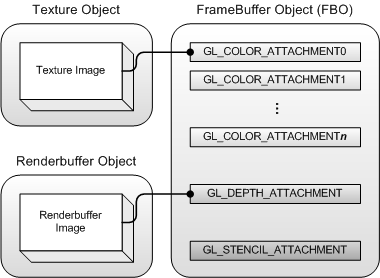
\includegraphics[height=33mm]{gl_fbo01.png}
		\end{center}		
	
		\Large
		\begin{itemize}
			\item renderování do textury - postprocessing
			\item generování pohledu na scénu
		\end{itemize}
								
	\end{frame}
	
	
	\begin{frame}[t,fragile]
		\frametitle{\textbf{Výsledky}}	

\begin{center}

		\begin{tabular}{lll}
			
\includegraphics[height=35mm]{blur.jpg} &		
			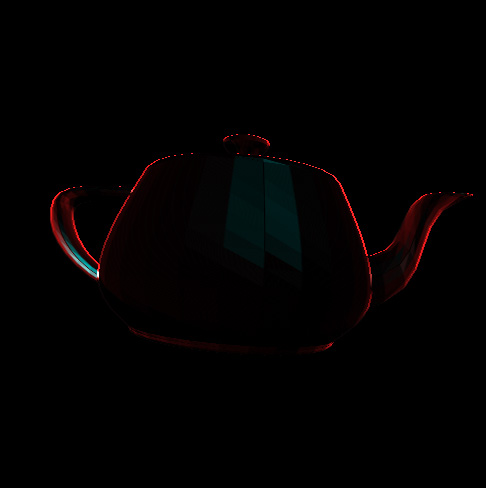
\includegraphics[height=35mm]{sobel.jpg} &
			
\includegraphics[height=35mm]{invert.jpg}
		\end{tabular}
		
		\vspace{10mm}
		viz. ukázka programu ... 
		
					\end{center}
		
	\end{frame}
	
	
\end{document} 
